\documentclass[a4paper,11pt]{article}
\usepackage[margin=21mm,headheight=16pt,footskip=11mm]{geometry}
\usepackage{fontspec}
\usepackage{kotex}
\setmainfont{DejaVu Sans}
\setmainhangulfont{NanumGothic}
\setsanshangulfont{NanumGothic}
\setmonofont[Scale=0.86]{DejaVu Sans Mono}
\setmonohangulfont{NanumGothic}
\usepackage{amsmath,amssymb,booktabs,tabularx,longtable,array}
\usepackage{tocloft}
\setlength{\cftsecnumwidth}{2.5em}
\setlength{\cftbeforesecskip}{3pt}
\setcounter{tocdepth}{1}
\renewcommand{\contentsname}{목차}
\usepackage{graphicx,tikz,xcolor,fancyhdr,fancyvrb,enumitem}
\usetikzlibrary{arrows.meta,positioning,calc,fit}
\usepackage[most]{tcolorbox}
\usepackage[unicode,colorlinks=true,linkcolor=blue!45!black,urlcolor=blue!55!black]{hyperref}
\hypersetup{pdftitle={RISC-V SIMT GPU 설계 상세 해설},pdfauthor={FPGA LAB},pdfsubject={1 SM, 4 Warp, 8 Thread per Warp on A7-Lite 200T},bookmarksdepth=2}
\definecolor{navy}{HTML}{16324F}
\definecolor{teal}{HTML}{007F86}
\definecolor{pale}{HTML}{EDF5F8}
\definecolor{ink}{HTML}{263444}
\setlength{\parindent}{0pt}
\setlength{\parskip}{6pt}
\linespread{1.19}
\setlist{nosep,leftmargin=1.8em,topsep=4pt}
\renewcommand{\arraystretch}{1.35}
\newcolumntype{Y}{>{\raggedright\arraybackslash}X}
\newcommand{\code}[1]{\texttt{\detokenize{#1}}}
\newcommand{\chapterpage}[1]{\clearpage\section{#1}}
\newcommand{\source}[1]{\par{\small\color{teal}구현 위치: \urlstyle{same}\path{#1}}\par}
\newtcolorbox{keybox}[1][]{colback=pale,colframe=teal,boxrule=0.6pt,arc=2mm,title=#1,fonttitle=\bfseries,breakable}
\DefineVerbatimEnvironment{Code}{Verbatim}{fontsize=\small,frame=single,framesep=6pt,rulecolor=\color{teal},baselinestretch=1.04}
\pagestyle{fancy}
\fancyhf{}
\fancyhead[L]{\small\color{navy}RISC-V SIMT GPU · 설계 상세 해설}
\fancyhead[R]{\small A7-Lite 200T}
\fancyfoot[L]{\small 1 SM / 4 Warp / 8 Thread}
\fancyfoot[R]{\thepage}
\begin{document}
\begin{titlepage}
\color{navy}
\vspace*{15mm}
{\large FPGA LAB · 구현과 검증을 함께 읽는 설계 문서}\par
\vspace{15mm}
{\Huge\bfseries RISC-V SIMT GPU}\par
\vspace{5mm}
{\LARGE 설계 상세 해설}\par
\vspace{9mm}
{\Large 1 SM · 4 Warp · Warp당 8 Thread}\par
\vspace{12mm}
\begin{tikzpicture}[>=Latex]
\foreach \x in {0,...,3} {
 \node[draw=teal,fill=pale,rounded corners,minimum width=31mm,minimum height=12mm] (w\x) at (\x*3.6,0) {Warp \x};
}
\node[draw=navy,fill=navy,text=white,rounded corners,minimum width=139mm,minimum height=15mm] (s) at (5.4,-2) {공유 스케줄러 · 명령 디코더};
\foreach \x in {0,...,3} {\draw[->,thick,teal] (w\x) -- (w\x|-s.north);}
\foreach \x in {0,...,7} {
 \node[draw=teal,fill=pale,minimum width=14mm,minimum height=10mm] (a\x) at (-0.9+\x*1.8,-4) {ALU \x};
 \draw[->,teal] (a\x|-s.south) -- (a\x);
}
\end{tikzpicture}
\vfill
\begin{keybox}[이 문서의 기준]
\code{docs/architecture.md}를 출발점으로 실제 RTL, 커널, 테스트벤치, Vivado 리포트와 보드 수신 결과를 대조해 확장했다. 일반 GPU의 모든 기능을 설명하는 문서가 아니라, 이 프로젝트에서 구현한 SIMT 구조가 어떻게 동작하는지 설명하는 해설서다.
\end{keybox}
\vspace{4mm}
{\large Microphase A7-Lite · XC7A200T-FBG484-2}\par
{\normalsize 문서 기준일: 2026년 10월 23일\quad /\quad Vivado 2022.1}\par
\end{titlepage}
\tableofcontents

\chapterpage{읽기 안내: 무엇을 이해하게 되는가}
이 설계에서 실행 가능한 thread는 32개지만, 물리 정수 ALU는 8개다. 이 두 숫자가 다른 이유를 이해하는 것이 출발점이다. thread는 프로그램이 사용하는 실행 문맥이고, lane은 실제 데이터를 계산하는 하드웨어 자리다. 4개 warp의 문맥을 보관해 두고, 스케줄러가 그중 하나를 골라 같은 8개 lane에 연결한다.

이 문서는 다음 질문을 순서대로 해결한다. 어떤 상태를 thread별로 저장하는가? 명령 하나를 실행할 때 어떤 상태를 거치는가? 같은 warp 안에서 분기 결과가 다르면 PC 하나로 어떻게 두 경로를 실행하는가? 왜 shared memory를 사용한 뒤 barrier가 필요한가? 마지막으로 실제 FPGA에서 무엇을 검증했는가?
\subsection{용어의 의미}
\par\medskip
\begin{tabularx}{\linewidth}{p{30mm}Y}
\toprule 용어 & 이 프로젝트에서의 의미 \\\midrule
Thread & 독립 레지스터 값을 가지는 논리적 작업 단위. 독립 fetch/decode나 PC는 없다.\\
Warp & PC, active mask, 분기 스택을 공유하는 8개 thread의 묶음.\\
Lane & 선택된 warp의 thread 하나를 처리하는 물리 연산 경로. 총 8개.\\
SM & scheduler, decoder, 8개 lane, 메모리와 제어기를 묶은 실행 장치.\\
Block & 함께 launch되고 BAR에 참여하는 32개 thread. 현재는 block 하나만 실행.\\
SIMT & 같은 명령을 여러 thread의 데이터에 적용하고 mask로 참여 thread를 제어하는 방식.\\
\bottomrule
\end{tabularx}
\par\medskip
\subsection{세 가지 근거를 구분해서 읽기}
\textbf{설계 규칙}은 RTL과 ISA 확장으로 정한 동작이다. \textbf{시뮬레이션 결과}는 테스트벤치에서 관측한 값이다. \textbf{실물 결과}는 보드에서 UART로 받아 확인한 값이다. 예를 들어 56,352클럭은 시뮬레이션 관측값이며 보드에서 별도 타이머로 측정한 값은 아니다.

각 절의 구현 위치를 따라 소스를 읽을 수 있다. 처음에는 전체 구조와 마스크 예제를 읽고, 이후 FSM과 메모리 절을 RTL과 함께 읽는 순서를 권한다. 코드의 상태명과 신호명은 원문을 유지했다.

\chapterpage{설계 사양과 병렬성의 의미}
\par\medskip
\begin{tabularx}{\linewidth}{p{53mm}Y}
\toprule 항목 & 사양 \\\midrule
SM / resident warp / thread & 1 / 4 / warp당 8, 총 32 thread\\
물리 연산부 & 정수 ALU 8개, 공유 decoder 1개\\
thread당 레지스터 & 32개 × 32비트. x0는 항상 0\\
register file 전체 & 32 thread × 32 registers × 4 bytes = 4 KiB\\
warp당 제어 상태 & 32-bit PC, 8-bit mask, 8-entry SIMT stack\\
메모리 & instruction ROM 4 KiB, global 32 KiB, shared 4 KiB\\
발행 방식 & single-issue, 비파이프라인, blocking LSU\\
기본 클럭 & 보드 50 MHz 입력, SM 10 MHz\\
\bottomrule
\end{tabularx}
\par\medskip
\subsection{동시에 보관하는 문맥과 동시에 계산하는 데이터}
32개 thread의 레지스터 값은 동시에 존재한다. 그러나 한 EXEC에서 계산되는 것은 선택된 warp의 최대 8개 thread다. 네 warp가 각자 별도 ALU 8개를 소유하는 구조가 아니다. warp 전환은 데이터 복사가 아니라 레지스터 파일 주소의 warp 부분과 warp PC 선택을 바꾸는 동작이다.

각 warp가 모두 runnable이고 메모리 명령이 없다면, W0의 명령 하나 다음에 W1, W2, W3의 명령 하나가 순서대로 처리된다. 일반 명령은 PICK/FETCH/EXEC의 3클럭을 사용하므로 한 warp가 다시 선택되는 간격은 이 단순 상황에서 약 12클럭이다.
\subsection{어떤 GPU 특성을 구현했는가}
명령 공유, thread별 데이터, warp scheduling, 마스크를 이용한 분기 실행, 재합류 스택, block barrier를 구현했다. 반면 여러 명령의 중첩 실행, 비차단 메모리, cache, texture, 부동소수점, 그래픽 API는 없다. 따라서 이 설계의 핵심은 GPU의 제어 구조를 작게 구현하고 관찰 가능하게 만드는 데 있다.
\begin{keybox}[성능 수치 해석]
ALU 8개라는 사실만으로 매 클럭 8개의 유효 thread 명령이 완료된다고 계산하면 안 된다. 일반 명령의 3클럭 제어 비용, 비활성 lane, 메모리 직렬 처리, SSY/JOIN과 분기 명령의 비용을 함께 고려해야 한다.
\end{keybox}

\chapterpage{전체 데이터 경로와 모듈 계층}
\begin{center}
\begin{tikzpicture}[>=Latex,node distance=9mm and 9mm,
 box/.style={draw=teal,fill=pale,rounded corners,align=center,text width=43mm,minimum height=12mm,font=\small}]
\node[box] (ctx) {4 warp contexts\\PC / mask / stack};
\node[box,right=of ctx] (sched) {Round-robin\\scheduler};
\node[box,below=of sched] (decode) {공유 instruction ROM\\fetch / decode};
\node[box,below=of ctx] (rf) {8 register banks\\warp별 문맥 선택};
\node[box,below=of decode] (alu) {8 ALU lanes\\mask에 따라 결과 기록};
\node[box,below=of rf] (branch) {분기 비교 / SSY / JOIN\\warp 상태 갱신};
\node[box,below=of alu] (lsu) {Blocking LSU\\lane 0 → 7 순차 처리};
\node[box,below=of branch] (shared) {4 KiB shared RAM};
\node[box,below=of lsu] (global) {32 KiB global RAM};
\node[box,below=of shared] (host) {Host read / UART};
\draw[->] (ctx)--(sched); \draw[->] (sched)--(decode);
\draw[->] (decode)--(alu); \draw[->] (rf)--(alu);
\draw[->] (alu)--(branch); \draw[->] (branch.west) -- ++(-.4,0) |- (ctx.west);
\draw[->] (alu)--(lsu); \draw[<->] (lsu)--(global);
\draw[<->] (lsu)--(shared); \draw[->] (global)--(host);
\end{tikzpicture}
\end{center}
명령어는 하나의 \code{insn} 레지스터에 들어간다. decoder가 만든 \code{alu}, \code{imm}, \code{rs1}, \code{rs2}, \code{rd}는 모든 lane에 공통이다. 반면 \code{a[g]}, \code{b[g]}, \code{result[g]}는 lane별 신호다. 같은 ADD를 수행해도 서로 다른 두 값을 더하므로 결과도 thread마다 다르다.
\begin{Code}
a7_gpu_top
  demo : gpu_demo
    gpu : compute_gpu
      sm : simt_sm
        decode : simt_decode
        lanes[0..7].rf   : simt_regfile
        lanes[0..7].unit : simt_alu
\end{Code}
\code{gpu_demo}는 자동 launch와 UART 전송을 담당하고, 실제 SIMT 실행은 \code{simt_sm} 내부에서 일어난다. 예전 \code{rv32i_core.v}는 기준 테스트용이며 새 top의 연산 코어로 인스턴스화되지 않는다.
\source{rtl/compute_gpu.sv, rtl/simt_sm.sv, rtl/gpu_demo.sv}

\chapterpage{Thread ID와 레지스터 파일 주소}
thread ID는 다음과 같이 결정된다.
\[
\mathrm{tid}=8\times\mathrm{warp\_id}+\mathrm{lane\_id}
\]
\par\medskip
\begin{tabularx}{\linewidth}{p{22mm}YYYY}
\toprule & W0 & W1 & W2 & W3 \\\midrule
lane 0 & tid 0 & tid 8 & tid 16 & tid 24\\
lane 1 & tid 1 & tid 9 & tid 17 & tid 25\\
lane 7 & tid 7 & tid 15 & tid 23 & tid 31\\
\bottomrule
\end{tabularx}
\par\medskip
물리 lane 하나의 register bank는 128 words다. 주소는 2비트 warp ID와 5비트 register ID를 이어 붙인 7비트 값이다.
\[
\mathrm{RF\ address}=32\times\mathrm{warp\_id}+\mathrm{register\_id}
\]
예를 들어 tid 19는 warp 2, lane 3이다. 이 thread의 x5는 \code{lanes[3].rf}의 주소 $2\times32+5=69$에 있다. tid 3도 같은 물리 bank를 사용하지만 warp 0이므로 x5의 주소는 5다. 따라서 값이 충돌하지 않는다.
\subsection{읽기와 쓰기}
\code{simt_regfile}은 두 소스 레지스터를 조합적으로 읽고, 상승 에지에서 한 목적 레지스터를 쓴다. 소스 번호가 0이면 RAM 내용 대신 상수 0을 내보낸다. 정상 명령의 목적 번호가 0이면 SM이 write enable을 꺼서 x0 쓰기를 무시한다.

ALU 결과를 기록할 때는 활성 lane만 \code{rf_we[g]}가 1이다. 비활성 lane에서도 조합 ALU 신호가 계산되거나 변할 수 있지만, 그 결과가 architectural register에 기록되지 않는다. 따라서 ``비활성''은 반드시 내부 모든 회로의 전원이 꺼진다는 뜻은 아니다.
\subsection{물리 저장량}
각 bank는 $128\times32=4096$ bits이고, 8개 bank의 합계는 32768 bits, 즉 4 KiB다. FPGA에서는 이 레지스터 파일을 LUT RAM으로 구현했다. 이 때문에 thread의 레지스터 수가 많아도 일반 flip-flop 사용량은 상대적으로 작다.
\source{rtl/simt_regfile.sv, rtl/simt_sm.sv}

\chapterpage{Launch, INIT, reset, 완료의 수명 주기}
\code{start}는 \code{busy=0}일 때만 수락한다. 수락한 상승 에지에서 busy를 1로 만들고 done, 오류, 통계 카운터를 초기화한다. 네 warp의 PC는 0, mask는 0xff, stack depth는 0으로 설정한다. busy 중 start는 무시하며 작업 큐에 저장하지 않는다.
\subsection{128클럭 초기화}
\code{init_index}가 0부터 127까지 증가하면서 8개 bank의 동일 주소를 동시에 쓴다. 한 클럭에 8개의 register word를 초기화하므로 전체 $8\times128$ words를 128클럭에 준비한다.
\par\medskip
\begin{tabularx}{\linewidth}{p{28mm}p{45mm}Y}
\toprule register & 시작 값 & 의미 \\\midrule
x2 / sp & $32768-256\times tid$ & thread별 stack의 위쪽 경계\\
x10 / a0 & tid & 0..31의 global thread ID\\
x11 / a1 & 32 & 전체 thread 수\\
x12 / a2 & 0 & global framebuffer base\\
그 외 & 0 & x0도 초기화되지만 읽기는 별도 상수 처리\\
\bottomrule
\end{tabularx}
\par\medskip
기존 register와 warp 상태는 새 launch에서 초기화된다. 반면 global/shared RAM은 보존된다. 커널이 읽기 전에 필요한 데이터를 기록해야 한다. ``이전 실행에서 사용하지 않은 RAM이 새 실행에서도 0일 것''이라고 가정하면 안 된다.
\subsection{종료와 오류 후 재시작}
EBREAK를 실행한 warp는 halted가 된다. 다른 warp는 계속 실행한다. PICK에서 네 warp의 halted가 모두 1임을 확인하면 busy를 내리고 done을 올린다. 정상 종료뿐 아니라 오류 정지도 halted에 포함되므로 done만 확인해서는 성공 여부를 알 수 없다. \textbf{done과 error를 함께 확인해야 한다.}

reset은 busy와 상태 머신을 초기 상태로 돌린다. 진행 중 memory instruction을 중단할 수 있지만 이미 이전 클럭에서 완료된 store를 되돌리지는 않는다. 새 launch는 오류와 stack 상태를 정리하므로 별도의 전원 재인가 없이 다시 실행할 수 있다.
\source{rtl/simt_sm.sv}

\chapterpage{FSM과 round-robin 스케줄러}
\begin{center}
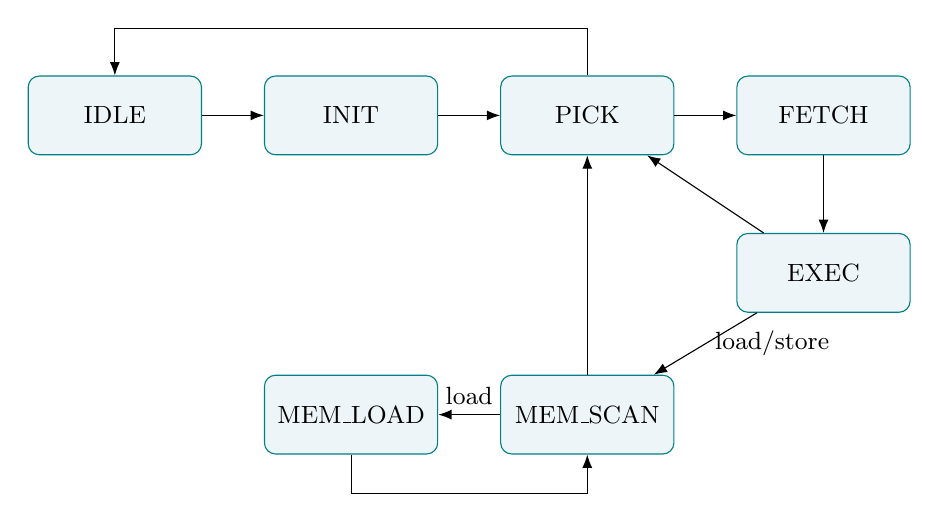
\begin{tikzpicture}[>=Latex,st/.style={draw=teal,fill=pale,rounded corners,minimum width=22mm,minimum height=10mm,font=\small}]
\node[st](idle)at(0,0){IDLE};\node[st](init)at(3,0){INIT};
\node[st](pick)at(6,0){PICK};\node[st](fetch)at(9,0){FETCH};
\node[st](exec)at(9,-2){EXEC};\node[st](scan)at(6,-3.8){MEM\_SCAN};
\node[st](load)at(3,-3.8){MEM\_LOAD};
\draw[->](idle)--(init);\draw[->](init)--(pick);\draw[->](pick)--(fetch);
\draw[->](fetch)--(exec);\draw[->](exec)--(pick);
\draw[->](exec)--node[right,font=\small]{load/store}(scan);
\draw[->](scan)--node[above,font=\small]{load}(load);
\draw[->](load.south)--++(0,-.5)-|(scan.south);
\draw[->](scan)--(pick);\draw[->](pick.north)--++(0,.6)-|(idle.north);
\end{tikzpicture}
\end{center}
\code{rr}은 다음 탐색 시작 warp를 나타낸다. 스케줄러는 rr부터 원형 순서로 네 후보를 조사하며, \code{halted=0}이고 \code{waiting=0}인 첫 후보를 선택한다. 선택한 warp가 k라면 rr은 $(k+1)\bmod4$가 된다.
\par\medskip
\begin{tabularx}{\linewidth}{p{25mm}Y}
\toprule 상태 & 주요 동작 \\\midrule
PICK & 완료 검사, barrier 해제 또는 deadlock 판정, runnable warp 선택\\
FETCH & 선택 warp PC의 범위/정렬 확인, instruction ROM에서 insn 저장\\
EXEC & decode, 연산, 분기, register write, memory 요청 준비\\
MEM\_SCAN & lane별 주소/데이터로 동기 RAM 접근 또는 inactive lane 건너뛰기\\
MEM\_LOAD & 직전 RAM 읽기 결과를 해당 lane의 목적 register에 기록\\
\bottomrule
\end{tabularx}
\par\medskip
일반 ALU 명령만 실행하고 네 warp가 모두 runnable이면 다음과 같은 순서가 된다.
\begin{Code}
cycle:  0    1     2     3    4     5     6    7     8
state: PICK FETCH EXEC  PICK FETCH EXEC  PICK FETCH EXEC
warp:   W0   W0    W0    W1   W1    W1    W2   W2    W2
\end{Code}
이것은 파이프라인 타이밍도가 아니다. W0 EXEC와 W1 FETCH가 겹치지 않는다. 따라서 한 warp의 명령이 완료될 때까지 다음 warp의 명령은 실행되지 않는다. LSU 중에는 PICK으로 돌아오지 않기 때문에 다른 warp로 메모리 지연을 숨기지도 못한다.
\source{rtl/simt_sm.sv}

\chapterpage{공유 decoder와 8개의 ALU}
\code{simt_decode}는 명령어 한 개를 받아 명령 종류(kind), ALU 연산 번호, immediate, 소스/목적 register 번호를 만든다. \code{kind}는 제어기가 무엇을 할지 결정하고, \code{alu}는 각 lane의 계산 종류를 결정한다. 둘은 서로 다른 제어 신호다.
\par\medskip
\begin{tabularx}{\linewidth}{p{18mm}p{35mm}Y}
\toprule alu 값 & 연산 & 의미 \\\midrule
0 / 1 & ADD / SUB & 32비트 덧셈/뺄셈, 상위 carry는 버림\\
2 & SLL & 왼쪽 shift, 이동량은 b[4:0]\\
3 / 4 & SLT / SLTU & signed/unsigned 비교 결과를 0 또는 1로 생성\\
5 & XOR & 비트별 exclusive OR\\
6 / 7 & SRL / SRA & 논리/산술 오른쪽 shift\\
8 / 9 & OR / AND & 비트별 논리 연산\\
10 & LUI & decoder가 만든 상위 immediate를 결과로 전달\\
11 & AUIPC & 현재 warp PC + 상위 immediate\\
\bottomrule
\end{tabularx}
\par\medskip
\subsection{공유되는 것과 lane별로 다른 것}
\begin{Code}
simt_alu unit(
    .op(alu),
    .a(a[g]),
    .b(immediate ? imm : b[g]),
    .pc(pc[current]),
    .y(result[g])
);
\end{Code}
위 인스턴스가 generate loop로 8개 생성된다. op와 PC, immediate는 공통이며, a와 register형 b는 lane별 값이다. ADDI라면 모든 lane이 같은 상수를 각자의 a에 더한다. ADD라면 각 lane의 두 register를 더한다.

load/store의 주소 계산과 JALR의 base+offset도 ALU의 덧셈을 사용한다. 반면 조건 분기의 비교는 SM 내부의 lane별 비교 로직에서 계산한다. 모든 연산이 \code{simt_alu}의 결과 y를 통해 이루어지는 것은 아니다.
\subsection{signed와 unsigned}
같은 32비트 0xffffffff라도 signed로는 -1, unsigned로는 4294967295다. SLT, BLT 등은 signed 비교를, SLTU, BLTU 등은 unsigned 비교를 한다. shift의 경우 SRA는 sign bit를 복제하고 SRL은 상위 비트를 0으로 채운다.
\source{rtl/simt_decode.sv, rtl/simt_alu.sv}

\chapterpage{명령 하나를 끝까지 따라가기: ADDI}
예를 들어 현재 선택된 warp가 W2이고 명령이 \code{addi x5,x6,7}이라고 하자. W2는 tid 16..23을 포함한다. 각 lane의 x6가 10, 20, 30, 40, 50, 60, 70, 80이고 mask=0xff이면 x5의 결과는 17, 27, 37, 47, 57, 67, 77, 87이다.
\subsection{PICK에서 EXEC까지}
\begin{enumerate}
\item PICK은 W2를 current로 선택한다. 다음 후보 탐색 시작점 rr은 W3가 된다.
\item FETCH는 \code{pc[2]}가 4바이트 정렬이고 4096 미만인지 확인한다. ROM word index는 PC를 4로 나눈 값이다.
\item insn에 저장된 ADDI를 decoder가 해석한다. kind=0, alu=0, rs1=6, rd=5, immediate=1, imm=7이다.
\item 각 lane의 RF는 W2의 x6, 즉 bank 내 주소 $2\times32+6=70$을 읽는다.
\item 8개 ALU가 각각 a+7을 계산한다. fault가 없고 rd가 0이 아니므로 rf\_we는 mask와 같아진다.
\item EXEC 종료 에지에서 W2의 x5 주소 69에 결과를 쓴다. W2의 PC는 4 증가하고 상태는 PICK으로 돌아간다.
\end{enumerate}
\subsection{mask가 0x55라면}
0x55는 이진수 01010101이며 lane 0,2,4,6만 활성이다. 이 경우 x5가 갱신되는 thread는 tid 16,18,20,22다. lane 1,3,5,7의 x5는 이전 값을 유지한다. 명령어를 4개로 나누는 것이 아니라 동일 명령에 대한 쓰기 참여를 선택하는 것이다.
\begin{keybox}[왜 scoreboard가 없는가]
이전 명령이 register write까지 끝난 뒤 다음 명령의 PICK/FETCH가 시작된다. 현재 구현에는 여러 명령이 동시에 진행되는 pipeline이나 미완료 load가 없으므로 그 사이의 register dependency를 추적하는 scoreboard가 필요하지 않다. 비차단 실행을 추가하면 이 전제가 달라진다.
\end{keybox}
\source{rtl/simt_sm.sv}

\chapterpage{분기가 어려운 이유와 active mask}
일반적인 scalar CPU thread는 자신의 PC를 따라 한 경로를 실행한다. 그러나 이 설계에서는 warp의 8개 thread가 PC 하나를 공유한다. 일부 thread가 if의 참 경로를, 다른 thread가 거짓 경로를 선택해도 두 PC를 동시에 fetch할 수 없다. 따라서 두 경로를 순차 실행하고, 각 경로에 속한 thread만 활성화한다.
\begin{Code}
if (tid % 2 == 0)
    x = 10;
else
    x = 20;
y = x + 1;
\end{Code}
위 코드는 설명용 의사 코드다. 일반 GCC가 이 프로젝트의 SSY/JOIN을 자동 삽입하지는 않는다. 실제 assembly에서는 합류 지점을 명시해야 한다.
\subsection{마스크의 bit 순서}
\par\medskip
\begin{tabularx}{\linewidth}{p{25mm}p{40mm}Y}
\toprule mask & bit 7 ... bit 0 & 활성 lane \\\midrule
0xff & 11111111 & 0,1,2,3,4,5,6,7\\
0x55 & 01010101 & 0,2,4,6\\
0xaa & 10101010 & 1,3,5,7\\
0x11 & 00010001 & 0,4\\
0x44 & 01000100 & 2,6\\
\bottomrule
\end{tabularx}
\par\medskip
현재 활성 mask를 M, 그중 조건이 참인 thread의 mask를 T라 하자. RTL은 inactive lane의 taken bit를 0으로 둔다. 따라서 T는 항상 M의 부분집합이고, 거짓 경로의 mask는 $F=M\mathbin{\&}\mathord{\sim}T$이다.
\begin{itemize}
\item T=0: 모두 거짓이다. PC+4로 진행하며 새 경로를 저장하지 않는다.
\item T=M: 모두 참이다. branch target으로 이동하며 분기 경로를 나누지 않는다.
\item 그 외: divergence다. T로 taken 경로를 실행하고 F와 fall-through PC를 보관한다.
\end{itemize}
\subsection{재합류 위치를 별도로 알려주는 이유}
RISC-V branch 명령에는 조건과 참일 때의 점프 오프셋만 들어 있다. if/else의 두 경로가 어디에서 다시 만나는지에 대한 구조 정보는 없다. 이 설계는 프로그램이 SSY로 합류 위치를 알려주고, JOIN을 실행했을 때 경로 전환 또는 mask 복원을 수행하도록 했다. 합류가 없으면 이후 공통 코드를 한쪽 thread만 실행하거나 같은 thread가 중복 실행할 수 있다.

\chapterpage{SSY/JOIN/BAR 인코딩과 assembler macro}
세 명령은 RISC-V custom-0 opcode 0x0b를 사용한 프로젝트 전용 확장이다. 표준 RISC-V 명령이나 특정 상용 GPU의 기계어와 호환되는 명령이 아니다.
\begin{Code}
.macro SSY target
    .word (((\target - .) & 0xfff) << 20) | 0x0000000b
.endm
.macro JOIN
    .word 0x0000100b
.endm
.macro BAR
    .word 0x0000200b
.endm
\end{Code}
\code{.macro}는 assembly 텍스트를 확장하고 \code{.word}는 32비트 값을 출력한다. SSY 한 번을 쓰면 위 수식으로 계산한 32비트 명령 하나가 ROM에 들어간다. \code{\target}은 인자 label, 점 하나인 \code{.}는 현재 SSY의 주소다. 둘의 차이는 명령 개수가 아니라 바이트 거리다.
\par\medskip
\begin{tabularx}{\linewidth}{p{30mm}p{35mm}Y}
\toprule 필드 & 비트 위치 & SSY 값 \\\midrule
immediate & [31:20] & target - 현재 PC의 하위 12비트\\
rs1 & [19:15] & 0\\
funct3 & [14:12] & 0; JOIN은 1, BAR는 2\\
rd & [11:7] & 0\\
opcode & [6:0] & 0x0b\\
\bottomrule
\end{tabularx}
\par\medskip
예를 들어 SSY가 0x100, JOIN이 0x120이면 거리는 0x20, 즉 32바이트다. 명령어 계산은 다음과 같다.
\[ (0x20\ll20)\,|\,0x0b=0x0200000b \]
 하드웨어는 immediate를 부호 확장한 뒤 현재 PC에 더해 0x120을 복원한다.
\begin{keybox}[범위 검사는 마스크 연산과 다르다]
12비트 signed 표현 범위는 -2048..2047이지만, 현재 SSY는 양수·4바이트 정렬만 허용하므로 거리는 4..2044바이트다. 또한 target은 ROM 범위 안이어야 한다. 매크로의 \code{& 0xfff}는 상위 비트를 버릴 뿐 범위를 검사하지 않는다. 큰 오프셋은 다른 양수로 잘릴 수도 있으므로 소스 작성자가 범위를 지켜야 한다.
\end{keybox}
\source{firmware/simt.inc, rtl/simt_decode.sv}

\chapterpage{SIMT 스택: 한 번의 분기를 정확히 추적하기}
SSY는 frame을 하나 push하고, 그 frame 안에서 한 번의 divergent branch를 관리한다. frame에는 다섯 종류의 정보가 있다.
\par\medskip
\begin{tabularx}{\linewidth}{p{35mm}p{18mm}Y}
\toprule 필드 & 폭 & 의미 \\\midrule
join\_pc & 32 bit & JOIN이 실행되어야 하는 주소\\
saved\_mask & 8 bit & SSY 진입 당시 참여 thread\\
pending\_pc & 32 bit & 아직 실행하지 않은 fall-through 경로 주소\\
pending\_mask & 8 bit & 해당 대기 경로의 참여 thread\\
split\_used & 1 bit & 이 frame에서 이미 divergent branch를 처리했는지\\
\bottomrule
\end{tabularx}
\par\medskip
다음은 주소를 명시한 설명용 예제다. 분기 조건은 홀수 lane에서 참이라고 가정한다.
\begin{Code}
0x100: SSY merge       # merge = 0x118
0x104: bne t0,zero,B
0x108: addi x5,zero,10
0x10c: j merge
0x110: B: addi x5,zero,20
0x114: j merge
0x118: merge: JOIN
0x11c: addi x6,x5,1
\end{Code}
\par\medskip
\begin{tabularx}{\linewidth}{p{20mm}p{18mm}Y}
\toprule 실행 PC & mask & 동작 \\\midrule
0x100 & ff & saved=ff, join=118, pending mask=0, split used=0으로 push\\
0x104 & ff & taken=aa. pending PC=108, pending mask=55 저장. split used=1\\
0x110 & aa & 홀수 lane의 x5만 20으로 변경\\
0x118 & aa & pending이 있으므로 PC=108, mask=55로 전환. pop하지 않음\\
0x108 & 55 & 짝수 lane의 x5만 10으로 변경\\
0x118 & 55 & pending이 0이므로 saved mask=ff 복원, frame pop\\
0x11c & ff & 모든 lane이 x6=x5+1 실행. 결과는 짝수 11, 홀수 21\\
\bottomrule
\end{tabularx}
\par\medskip
첫 JOIN에서 pending mask를 지우지만 split used는 유지한다. 따라서 같은 frame의 두 번째 경로에서 새로운 divergent branch가 나타나면 오류다. 그 분기를 중첩하려면 별도의 SSY가 필요하다. 모든 thread가 같은 경로를 선택했더라도 SSY를 실행했다면 JOIN으로 frame을 정리해야 한다.

\chapterpage{중첩 분기: selftest의 마스크와 stack depth}
\code{selftest_simt.S}는 tid bit 0으로 짝수/홀수를 나눈 뒤, 각 경로에서 bit 1로 다시 나눈다. 각 warp의 tid 시작값이 8의 배수이므로 lane별 분류는 네 warp에서 같다.
\begin{center}
\begin{tikzpicture}[>=Latex,b/.style={draw=teal,fill=pale,rounded corners,align=center,minimum width=25mm,minimum height=10mm}]
\node[b](root)at(5,0){ff / depth 0};
\node[b](odd)at(2.5,-1.5){aa / depth 1};\node[b](even)at(7.5,-1.5){55 / depth 1};
\node[b](a)at(1,-3){88 / 400};\node[b](b)at(4,-3){22 / 300};
\node[b](c)at(6,-3){44 / 200};\node[b](d)at(9,-3){11 / 100};
\draw[->](root)--node[left,font=\small]{먼저}(odd);\draw[->](root)--node[right,font=\small]{나중}(even);
\draw[->](odd)--(a);\draw[->](odd)--(b);\draw[->](even)--(c);\draw[->](even)--(d);
\end{tikzpicture}
\end{center}
도식 아래쪽 숫자는 mask와 s2 결과다. leaf 경로에서는 내부 SSY까지 쌓였으므로 stack depth가 2다. taken-first 순서로 88,22,44,11의 thread 묶음이 실행된다.
\begin{enumerate}
\item outer SSY가 saved mask=ff를 저장한다. 외부 BNE는 홀수 aa를 먼저 선택하고 짝수 55를 대기시킨다.
\item odd SSY가 saved mask=aa를 저장한다. 내부 BNE는 bit 1이 1인 88을 먼저 실행해 s2=400을 쓴다.
\item odd JOIN의 첫 실행에서 22로 전환해 s2=300을 쓴다. 두 번째 실행에서 mask=aa, depth=1로 복귀한다.
\item outer JOIN은 pending인 짝수 55로 전환한다. even SSY 아래에서 44는 200, 11은 100을 기록한다.
\item even JOIN이 55를 복원하고, 마지막 outer JOIN이 ff와 depth=0을 복원한다.
\end{enumerate}
최종 s2는 lane 0..7 순서로 100,300,200,400,100,300,200,400이다. 각 lane이 자기 register 값을 보존했으므로 마지막 전체-mask store에서 이 값들을 동시에 결과로 내보낼 수 있다.
\subsection{스택 저장소의 분리}
RTL은 네 warp의 스택을 32-entry 배열로 저장하며 \code{warp*8+depth}로 push 위치를 계산한다. top은 \code{warp*8+depth-1}이다. 중첩 깊이는 warp별로 독립적이고 8을 넘는 push는 오류 17이다. register의 software stack과 이 SIMT control-flow stack은 전혀 다른 저장소다.
\source{firmware/selftest_simt.S}

\chapterpage{제어 흐름의 허용 범위와 주의할 프로그램}
\subsection{Uniform branch와 uniform loop}
같은 warp의 모든 active thread가 같은 판단을 하면 PC를 한 방향으로만 옮길 수 있다. 이 경우 새로운 pending path가 생기지 않으므로 SSY가 필요하지 않다. selftest의 도착 지연 loop는 warp별 횟수는 다르지만 같은 warp 안에서는 횟수가 같아 uniform하다. ``warp마다 다르다''와 ``warp 내부에서 다르다''를 구분해야 한다.

render 커널도 thread당 128픽셀을 처리하므로 loop 탈출은 uniform하다. 반면 thread별 입력 데이터에 따라 반복 횟수가 다른 loop는 한 frame 안에서 반복적으로 split될 수 있다. 현재의 one-split-per-frame 규칙으로 임의의 C while loop를 그대로 처리할 수는 없다. compiler의 control-flow 변환이나 다른 실행 모델이 필요하다.
\subsection{JAL과 JALR}
JAL은 공통 PC-relative target으로 이동하고 활성 lane의 rd에 PC+4를 쓴다. JALR은 각 active lane에서 base+immediate를 계산하고 bit 0을 지운다. 그 결과가 모두 같아야 warp PC 하나로 이동할 수 있다. target이 lane마다 다르면 오류 19다. target의 bit 1이 1이면 여전히 4바이트 비정렬이므로 오류 0x80이 된다.
\subsection{부분 종료와 barrier}
EBREAK는 mask=ff이고 stack depth=0일 때만 정상 종료한다. 일부 thread만 먼저 종료하는 기능은 없다. BAR도 같은 조건을 요구한다. divergent region 내부에서 ``이쪽 경로 thread만 barrier를 기다리자''고 하면 다른 경로를 실행할 thread와 충돌하므로 오류로 막는다.
\begin{keybox}[세 가지 다른 상황]
\textbf{경로 합류}: 같은 warp 안에서 SSY/JOIN으로 mask를 복원한다.\par
\textbf{Block 동기화}: 네 warp가 BAR로 같은 지점에 도착했는지 확인한다.\par
\textbf{프로그램 종료}: full-mask EBREAK로 해당 warp를 halted 상태로 만든다.
\end{keybox}
SSY가 저장한 주소가 실제 JOIN 명령인지 push 시점에 미리 검증하지는 않는다. JOIN을 실행할 때 현재 PC와 저장한 join PC의 일치를 검사한다. 잘못된 커널이 JOIN 자체를 건너뛰고 무한 루프를 돌면 자동 검출을 보장하지 않는다.

\chapterpage{메모리 맵과 주소 계산}
명령 ROM과 데이터 RAM은 Harvard 방식으로 분리되어 있다. 명령 PC=0은 ROM의 첫 명령을 뜻하고, load/store 주소 0은 global RAM의 첫 word를 뜻한다. 같은 숫자라도 접근 경로가 다르다. ROM을 load로 직접 읽거나 코드에 둔 상수를 global RAM 초기값으로 사용하는 기능은 없다.
\par\medskip
\begin{tabularx}{\linewidth}{p{56mm}p{20mm}Y}
\toprule 바이트 주소 & 크기 & 용도 \\\midrule
0x00000000..0x00003fff & 16 KiB & framebuffer 4096개 × 4바이트\\
0x00004000..0x00005fff & 8 KiB & scratch / 테스트 결과\\
0x00006000..0x00007fff & 8 KiB & thread별 software stack 예약 영역\\
0x10000000..0x10000fff & 4 KiB & block 전체 shared memory\\
\bottomrule
\end{tabularx}
\par\medskip
전체 global RAM은 8192 words다. 주소가 유효하다고 확인한 뒤 word 선택에는 \code{addr[14:2]}를 사용한다. shared RAM은 1024 words이고 \code{addr[11:2]}를 사용한다. low 2 bits는 word 안의 byte 위치다.

하드웨어는 이 주소 범위와 정렬을 검사하지만, framebuffer/scratch/stack의 소프트웨어 구분은 보호하지 않는다. 예를 들어 stack이 너무 크게 자라 다른 thread의 영역을 덮어써도 32 KiB 안이라면 접근 오류가 아닐 수 있다.
\subsection{Stack 시작 주소의 예}
sp는 $0x8000-256\times tid$이다. tid 0의 sp는 0x8000이고 사용 가능한 예약 구간은 0x7f00..0x7fff다. tid 31의 sp는 0x6100이고 예약 구간은 0x6000..0x60ff다. 일반적인 하향 성장 stack처럼 store 전에 sp를 감소시켜야 한다. sp의 초기값 자체는 영역의 위쪽 경계다.
\subsection{Host 읽기}
\code{host_word}는 byte 주소가 아닌 word index다. byte 주소 0x4000을 읽으려면 host word 4096을 넣는다. RAM 값과 bounds-valid를 상승 에지에서 등록하므로 결과는 동기식 1클럭 읽기다. 8192 이상은 0을 반환한다. busy 중 읽기 자체는 존재하지만 GPU write와의 같은 주소 충돌 값에 의존하지 말고 done 이후 결과를 사용해야 한다.

\chapterpage{LSU: 주소 검증부터 실제 commit까지}
LSU는 Load/Store Unit의 약자다. 이 설계의 LSU는 8개 lane의 요청을 순서대로 RAM에 전달한다. 주소가 서로 연속적이어도 하나의 큰 전송으로 합치는 coalescing은 하지 않는다.
\subsection{먼저 모든 active lane을 검사한다}
EXEC에서 각 lane의 유효 주소를 계산한다. active mask가 1인 lane에 대해서만 범위와 정렬을 검사한다. byte는 어떤 주소도 가능하고 halfword는 2바이트, word는 4바이트 정렬이 필요하다. 하나라도 위반하면 그 warp를 fault 처리하고 memory transaction을 시작하지 않는다.

예를 들어 lane 0..6은 정상 주소이고 lane 7만 잘못된 주소라면, lane 0부터 일부 store를 수행한 뒤 나중에 실패하는 방식이 아니다. 처음부터 전체 명령의 store를 억제한다. 이는 주소 오류에 대해 부분 쓰기를 피하는 규칙이며, reset에 대한 rollback이나 atomic 연산을 의미하지는 않는다.
\subsection{검사 후 요청을 고정한다}
주소 8개, store data 8개, mask, load/store 구분, funct3와 load 목적 register를 latch한다. 이후 MEM\_SCAN은 0..7번 lane을 순서대로 조사한다. inactive lane은 RAM에 접근하지 않고 다음 번호로 넘어간다.
\par\medskip
\begin{tabularx}{\linewidth}{p{25mm}Y}
\toprule 요청 & MEM\_SCAN에서의 처리 \\\midrule
Inactive & 접근 없이 mem\_lane 증가\\
Store & byte enable에 해당하는 RAM 바이트 기록, mem\_lane 증가\\
Load & 동기 RAM 읽기 결과를 q에 저장, MEM\_LOAD로 전환\\
Lane=8 & 전체 순회 완료. PICK으로 복귀\\
\bottomrule
\end{tabularx}
\par\medskip
MEM\_LOAD에서는 직전 읽기의 주소 하위 비트로 byte/halfword를 선택하고 필요한 부호 확장을 수행한다. 결과를 해당 lane의 rd에 쓴 뒤 lane 번호를 증가시키고 MEM\_SCAN으로 돌아간다. rd=x0이면 쓰기만 무시하며 주소 검증과 읽기 동작은 그대로 수행한다.
\source{rtl/simt_sm.sv}

\chapterpage{LSU의 클럭 수와 메모리 충돌}
한 명령의 기본 PICK/FETCH/EXEC에 3클럭이 필요하다. 그 뒤 MEM\_SCAN은 8개 lane과 종료 검사 한 번을 거치므로 9클럭이다. load는 활성 lane마다 MEM\_LOAD 한 클럭이 추가된다.
\[
C_{store}=3+9=12,\qquad C_{load}=3+9+A
\]
여기서 A는 active lane 수다. 이 식은 단일 memory instruction의 정상 상태 진행을 센 값이며 launch 초기화나 barrier 대기 시간은 포함하지 않는다.
\par\medskip
\begin{tabularx}{\linewidth}{p{37mm}p{35mm}Y}
\toprule 상황 & 추가 LSU 클럭 & 기본 3클럭 포함 \\\midrule
8 active lane store & 9 & 12\\
4 active lane store & 9 & 12\\
8 active lane load & 17 & 20\\
4 active lane load & 13 & 16\\
\bottomrule
\end{tabularx}
\par\medskip
마스크가 절반이어도 store의 scan 횟수는 줄지 않는다. inactive lane도 한 번씩 검사하기 때문이다. load에서는 비활성 lane에 대한 MEM\_LOAD를 생략하므로 active 수에 따라 시간이 줄어든다.
\begin{Code}
Full-mask load (after EXEC):
SCAN0 LOAD0 SCAN1 LOAD1 ... SCAN7 LOAD7 SCAN8 -> PICK

Mask 0x05 load (lanes 0,2 only):
SCAN0 LOAD0 SCAN1 SCAN2 LOAD2 SCAN3 ... SCAN7 SCAN8
\end{Code}
\subsection{같은 주소에 여러 thread가 쓰면}
하나의 vector store 안에서는 lane 0부터 7까지 처리하므로, 같은 주소에 쓰는 활성 lane 중 번호가 가장 큰 lane의 값이 마지막에 남는다. warp 사이의 순서는 scheduler의 실제 실행 순서에 따른다. 이 규칙을 알고 있어도 read-modify-write의 atomic성을 보장하는 것은 아니다.

global RAM은 별도 host read port를 가진다. host가 GPU와 같은 word를 동시에 읽고 쓰는 경우의 관측값은 프로그램 계약에 포함하지 않는다. 데이터를 안전하게 비교하려면 전체 작업이 끝난 done 상태에서 읽어야 한다.
\begin{keybox}[성능 한계의 위치]
다른 warp가 실행 가능해도 LSU가 한 명령을 처리하는 동안 scheduler는 멈춰 있다. 이 부분을 개선하려면 outstanding 요청, 응답의 warp/lane/rd 식별, scoreboard 및 실행 재개 규칙을 함께 설계해야 한다.
\end{keybox}

\chapterpage{Little-endian, byte enable, 부호 확장}
selftest는 각 thread의 작업 word에 0x80ff7f01을 저장한다. little-endian에서는 낮은 주소에 낮은 유효 바이트가 위치한다.
\par\medskip
\begin{tabularx}{\linewidth}{p{29mm}YYYY}
\toprule 주소 & base+0 & base+1 & base+2 & base+3 \\\midrule
저장 byte & 0x01 & 0x7f & 0xff & 0x80\\
\bottomrule
\end{tabularx}
\par\medskip
\subsection{같은 비트를 다르게 확장하기}
\par\medskip
\begin{tabularx}{\linewidth}{p{32mm}p{42mm}Y}
\toprule 명령 & 32-bit 결과 & 이유 \\\midrule
LB +3 & 0xffffff80 & byte 0x80의 sign bit를 상위 24비트에 복제\\
LBU +3 & 0x00000080 & 상위 24비트를 0으로 채움\\
LH +2 & 0xffff80ff & little-endian halfword 0x80ff의 sign bit 복제\\
LHU +2 & 0x000080ff & 상위 16비트를 0으로 채움\\
LW +0 & 0x80ff7f01 & word 전체를 그대로 반환\\
\bottomrule
\end{tabularx}
\par\medskip
\subsection{부분 store가 다른 바이트를 보존하는 방법}
SB로 base+1에 0xaa를 쓰면 byte enable은 0010이다. store data는 한 바이트만큼 왼쪽으로 이동하고, 해당 byte lane만 변경한다. 결과는 0x80ffaa01이다. 이어 SH로 base+2에 0x1234를 쓰면 byte enable은 1100이며 최종 word는 0x1234aa01이 된다.
\begin{Code}
mwrite = source_data << (byte_offset * 8)
SB: mstrb = 0001 << byte_offset
SH: mstrb = 0011 << byte_offset
SW: mstrb = 1111
\end{Code}
SH에서 byte offset=3은 두 바이트가 word 경계를 넘기 전에 정렬 검사에서 거부된다. SW의 하위 주소 두 비트가 0이 아니어도 거부된다. 현재 구현은 비정렬 접근을 여러 RAM 접근으로 분해해서 지원하지 않는다.

FPGA에서 global/shared RAM의 등록된 읽기 출력은 각각 분리되어 있다. 읽기 전에 여러 메모리를 큰 조합 mux로 합치면 Vivado가 원하는 BRAM 패턴을 인식하지 못할 수 있어, RAM별 q register를 두고 이후에 선택하도록 구현했다.
\source{rtl/simt_sm.sv}

\chapterpage{Shared memory와 BAR의 정확한 의미}
shared memory는 block의 모든 thread가 접근할 수 있는 4 KiB 데이터 저장소다. thread별 전용 저장소가 아니다. 서로 다른 주소를 쓰도록 index를 설계하고, 다른 thread의 데이터를 읽기 전에 필요한 동기화를 해야 한다.
\begin{Code}
shared[tid] = tid;
BAR;
value = shared[31 - tid];
\end{Code}
이 예제는 설명용 의사 코드이며 selftest에 실제 assembly로 구현되어 있다. tid 0은 31의 기록을, tid 31은 0의 기록을 읽는다. 따라서 같은 warp 안의 데이터만 확인하는 테스트가 아니다.
\subsection{먼저 도착한 warp의 상태}
BAR를 실행한 warp는 waiting bit를 1로 설정하고 barrier PC를 기록한다. PC 자체는 일반 EXEC 처리에 따라 이미 다음 명령을 가리키지만, waiting warp는 scheduler가 선택하지 않으므로 실제로 다음 명령을 실행하지 않는다.
\par\medskip
\begin{tabularx}{\linewidth}{p{35mm}p{25mm}Y}
\toprule 사건 & waiting[3:0] & 가능한 실행 \\\midrule
W0 도착 & 0001 & W1,W2,W3는 계속 실행\\
W1 도착 & 0011 & W2,W3 실행\\
W2 도착 & 0111 & W3 실행\\
W3 도착 & 1111 & 다음 PICK에서 barrier PC 비교\\
모든 PC 일치 & 0000 & 네 warp 모두 runnable로 복귀\\
\bottomrule
\end{tabularx}
\par\medskip
표는 도착 순서의 한 예이지 모든 프로그램에서의 고정 순서는 아니다. ``동시에 해제''는 같은 제어 에지에 waiting을 모두 지운다는 의미다. 이후 명령을 네 warp가 동시에 발행하는 것은 아니며, 여전히 round-robin으로 하나씩 선택한다.
\subsection{메모리 가시성이 확보되는 이유}
현재 LSU는 이전 store를 모두 완료한 뒤에야 다음 명령으로 진행한다. 그래서 warp가 BAR에 도착했다면 그 warp의 이전 메모리 요청은 끝나 있다. 네 warp 모두 도착한 뒤에는 이후 load가 다른 warp의 완료된 기록을 읽을 수 있다. 이것은 현재의 blocking 순차 구조에 기반한 설명이며, 비차단 LSU를 도입하면 별도의 요청 drain 또는 fence 조건을 설계해야 한다.

JOIN은 warp 내부 mask 복원이고 BAR는 block 전체의 도착 확인이다. JOIN 뒤라도 다른 warp가 shared memory 쓰기를 마쳤다는 보장은 없다. 반대로 BAR를 divergent region 안에 넣어 JOIN을 대신할 수도 없다.

\chapterpage{Barrier 오용과 deadlock 검출}
BAR는 mask=0xff, stack depth=0인 상태에서만 허용한다. 즉 해당 warp의 모든 8개 thread가 열린 분기 frame 없이 참여해야 한다. 정상 도착한 네 warp의 barrier PC도 같아야 한다.
\subsection{서로 다른 barrier 위치에 도착한 경우}
W0가 코드의 BAR A에서, W1..W3가 BAR B에서 기다리면 waiting은 1111이지만 barrier PC가 다르다. 하드웨어는 이를 정상 동기화로 풀어 주지 않고 모든 warp를 오류 22로 정지시킨다. 서로 관계없는 동기화 지점을 한 번의 barrier로 합치면 프로그램 순서가 깨지기 때문이다.
\subsection{일부 warp가 먼저 종료한 경우}
W0가 EBREAK로 종료하고 W1..W3가 BAR에서 기다리면, 모든 warp의 도착을 만족시킬 수 없다. scheduler가 선택할 runnable warp가 없고 waiting warp가 남아 있으면, 기다리던 warp를 오류 22로 정지시킨다. 이미 정상 종료한 W0에 새 오류를 붙이지는 않는다.
\subsection{검출되지 않는 무한 대기}
W0가 BAR에서 기다리는데 W1이 무한 루프를 계속 돌면 W1은 runnable이다. 따라서 ``실행 가능한 warp 없음'' 조건이 성립하지 않아 deadlock 판정은 발생하지 않는다. watchdog이나 명령 수 제한은 없다. 실제 시스템 통합 시에는 외부 timeout과 reset 정책을 추가할 수 있다.
\begin{keybox}[반복 barrier의 사용]
한 번 정상 해제되면 waiting은 모두 0이 된다. 다음 BAR 실행에서 각 warp가 다시 PC를 기록하므로 같은 barrier를 반복 사용할 수 있다. 그러나 하드웨어가 프로그램의 모든 동적 제어 흐름을 분석하는 것은 아니다. 같은 PC에서 서로 다른 loop 회차를 잘못 맞추는 프로그램 오류까지 일반적으로 판별하지는 않는다.
\end{keybox}
selftest는 warp별로 4/8/12/16회 지연 loop를 넣어 arrival을 어긋나게 만든다. 늦은 warp가 shared memory를 기록하기 전에 빠른 warp가 읽지 못하도록 기다리는지 확인한다. 반복 barrier 횟수와 실제 읽힌 데이터 모두를 검사해야 단순히 명령을 통과했다는 사실보다 강한 검증이 된다.
\source{rtl/simt_sm.sv}

\chapterpage{Fault 처리와 진단 코드}
오류가 생기면 해당 warp의 error와 halted를 설정하고 fault code를 저장한다. 명령의 register write와 memory 시작을 억제하며, EXEC/FETCH 오류에서는 PC를 더 진행시키지 않는다. 다른 runnable warp는 계속 실행한다. 예외 handler로 점프하거나 CSR에 원인을 저장하는 privileged RISC-V trap 체계는 구현하지 않았다.
\begin{longtable}{p{18mm}p{48mm}p{87mm}}
\toprule 코드 & 원인 & 확인할 내용 \\\midrule\endhead
0 & 오류 없음 & error bitmap도 함께 확인\\
1 & instruction fetch 범위 & 점프/복귀 target이 0..4095에 있는가\\
2 & illegal instruction & 지원하지 않는 opcode/funct 조합인가\\
4 / 5 & load 정렬 / 접근 & LH/LW 정렬, global/shared 범위\\
6 / 7 & store 정렬 / 접근 & SH/SW 정렬, active lane 전체 주소\\
11 & ECALL & 이 실행 환경에서는 오류 종료\\
16 & 잘못된 divergence & SSY 누락 또는 같은 frame에서 두 번째 split\\
17 & SIMT stack overflow & depth=8에서 SSY를 추가 실행했는가\\
18 & SSY/JOIN 오류 & SSY target 범위·정렬, JOIN underflow/PC 불일치\\
19 & divergent JALR & active lane의 indirect target이 같은가\\
20 & 잘못된 EBREAK & mask=ff이고 stack이 비었는가\\
21 & 잘못된 BAR & mask=ff이고 stack이 비었는가\\
22 & barrier 불일치/deadlock & 다른 PC에 도착했거나 종료 warp 때문에 막혔는가\\
0x80 & instruction 비정렬 & 선택된 target/현재 PC가 4바이트 정렬인가\\
\bottomrule
\end{longtable}
표에서 0x80을 제외한 코드는 10진수다. 0을 정상 상태로 사용하기 때문에 instruction misalignment는 표준 원인 번호 0 대신 이 인터페이스 전용 0x80으로 표시한다. 표의 숫자를 표준 machine-mode CSR 값이라고 가정하면 안 된다.
\subsection{Packed 출력 읽기}
\code{fault_codes[warp*8 +: 8]}에 8비트 원인이 들어간다. W1만 load 접근 오류라면 \code{error=4'b0010}, \code{fault_codes=32'h00000500}이다. 이 신호들은 SM의 진단 출력이며 현재 UART 프레임은 세부 코드 대신 4비트 error bitmap만 전송한다. BAR 대기 후 PICK에서 검출한 deadlock의 경우 PC는 이미 BAR+4일 수 있으며, 원래 동기화 위치는 barrier\_pc에 남아 있다.

FETCH에서 범위/정렬을 검사하고 EXEC에서는 명령별 오류를 검사한다. memory instruction에서 정렬과 범위를 동시에 위반하면 정렬 오류가 우선한다. branch target 정렬은 실제 taken 경로가 있을 때 검사한다. 테스트벤치는 이런 실패 뒤에 새 launch가 정상 동작하는지도 확인한다.

\chapterpage{Selftest를 결과 메모리와 연결해서 읽기}
selftest 커널은 global RAM에 결과를 쓰고 종료한다. PASS/FAIL은 테스트벤치가 판단한다. 검증 대상 커널이 스스로 ``성공''이라고 출력하는 구조가 아니라, 별도로 계산한 기대값과 결과를 비교한다.
\par\medskip
\begin{tabularx}{\linewidth}{p{23mm}p{29mm}Y}
\toprule byte base & host word base & thread t의 기대값 \\\midrule
0x0000 & 0 & t\%4=0/1/2/3이면 100/300/200/400\\
0x0080 & 32 & 다음 thread ((t+1)\&31)의 위 결과\\
0x0100 & 64 & 0xffffff80 (LB)\\
0x0180 & 96 & 0x00000080 (LBU)\\
0x0200 & 128 & 0xffff80ff (LH)\\
0x0280 & 160 & 0x000080ff (LHU)\\
0x0300 & 192 & 0x1234aa01 (SB/SH/LW)\\
0x0380 & 224 & 0 (x0 쓰기 무시)\\
0x0400 / 0x0480 & 256 / 288 & t==0 / t!=0\\
0x0500 / 0x0580 & 320 / 352 & signed 비교: t<16 / t>=16\\
0x0600 / 0x0680 & 384 / 416 & unsigned 비교: t>=16 / t<16\\
0x4000 & 4096 & 31-t (cross-warp shared 교환)\\
\bottomrule
\end{tabularx}
\par\medskip
각 배열의 host word index는 base+t이고 byte 주소는 base+4t다. 이 차이를 혼동하면 결과가 맞아도 잘못된 주소를 읽어 실패로 보일 수 있다.
\subsection{왜 unsigned 비교의 결과가 뒤집히는가}
t0=t-16을 사용한다. t가 0..15이면 signed로 -16..-1이지만 unsigned로는 0xfffffff0..0xffffffff다. 따라서 unsigned 16보다 크다. t가 16..31이면 t0는 0..15이므로 unsigned 16보다 작다.
\subsection{분기 통계의 기대값}
중첩 분기는 warp마다 외부 1회와 내부 두 경로의 1회씩, 총 3회 split을 만든다. 네 warp이므로 12회다. 추가 BEQ/BNE 검사는 warp 0에서만 true/false가 섞여 각각 1회씩 발생한다. 나머지 비교는 warp 내부에서 uniform이므로 전체 split 기대값은 14회, barrier release는 2회다.
\source{firmware/selftest_simt.S, sim/tb_simt_control.sv}

\chapterpage{64×64 렌더 커널과 UART 데이터 경로}
render 커널은 각 thread에 서로 다른 픽셀을 배정한다. thread t는 t, t+32, t+64, ... 위치를 처리한다. 전체 4096개 픽셀이 32 thread에 균등 배정되어 thread당 128개가 된다.
\[
x=p\mathbin{\&}63,\qquad y=p\gg6,\qquad \mathrm{pixel\ address}=4p
\]
커널은 x/y 그라데이션과 checker blue 값을 계산한 뒤, $|x-31|+|y-31|<16$이면 중앙 마름모 색으로 바꾼다. 이 조건은 lane마다 다를 수 있으므로 SSY/JOIN으로 감싼다. loop 반복 횟수는 같아 loop branch는 uniform하다.
\subsection{Global word 하나가 픽셀 하나}
픽셀은 0x00RRGGBB다. thread별 bank를 호스트가 다시 섞는 이전 manycore 방식과 달리, 지금은 커널이 최종 scan 순서의 global 주소에 직접 쓴다. UART는 done 이후 global word 0..4095를 차례로 읽는다.
\par\medskip
\begin{tabularx}{\linewidth}{p{31mm}Y}
\toprule UART byte 위치 & 내용 \\\midrule
0..3 & ASCII GPU2\\
4 / 5 / 6 & width=64 / height=64 / thread count=32\\
7 & warp error bitmap, 하위 4비트 사용\\
8..16391 & 4096개의 little-endian 32-bit pixel\\
\bottomrule
\end{tabularx}
\par\medskip
예를 들어 word 0x00ffc020은 UART에서 20 c0 ff 00 순서로 전송된다. Python 캡처 도구는 little-endian으로 word를 복원한 뒤 RGB byte를 꺼내 PPM 이미지로 저장한다.

UART는 8-N-1이므로 byte당 start 1, data 8, stop 1의 총 10비트가 필요하다. 10 MHz를 87로 나누므로 실제 baud는 약 114943이며 전체 16,392-byte frame 전송 시간은 약 1.426초다. 이후 약 1초의 gap을 두고 같은 완성 이미지를 반복 전송한다. 이것은 매번 커널을 다시 실행한다는 뜻이 아니다.
\source{firmware/render_simt.S, rtl/gpu_demo.sv, rtl/uart_tx.sv, scripts/frame.py}

\chapterpage{클럭, reset, FPGA 메모리 추론}
\subsection{50 MHz에서 10 MHz 만들기}
보드의 J19 핀으로 들어오는 50 MHz 클럭을 MMCM에 넣는다. 설정은 입력 분주 1, feedback 배수 20, 출력 분주 100이다.
\[
f_{VCO}=50\,\mathrm{MHz}\times20=1000\,\mathrm{MHz},\qquad
f_{SM}=1000/100=10\,\mathrm{MHz}
\]
feedback과 GPU 클럭 경로에 BUFG를 각각 하나씩 사용한다. RTL 카운터 출력으로 새 클럭을 만드는 대신 FPGA의 전용 클럭 자원을 사용한 것이다.
\subsection{Reset 경로}
MMCM locked가 낮아지면 4-bit reset chain은 비동기적으로 1111이 된다. locked가 높아지면 GPU 클럭에 따라 0을 밀어 넣어 해제한다. 그 뒤 별도의 \code{gpu_reset} 레지스터를 한 단계 더 거쳐 SM으로 전달한다. 따라서 SM과 BRAM 제어에 들어가는 최종 reset 변화는 GPU 클럭 에지에 맞춰진다.

이 설계의 reset은 RAM 전체를 0으로 지우지 않는다. 큰 RAM에 reset loop를 넣으면 BRAM 추론을 방해할 수 있고, 원래 의도한 ``launch 시 메모리 유지'' 규칙과도 맞지 않는다. FPGA 구성 시 초기값과 runtime reset을 구분해야 한다.
\subsection{왜 NoBramPowerOpt를 적용했는가}
초기 구현에서는 등록된 RAM 출력의 형태 때문에 LUT RAM으로 추론되었다. RAM별 synchronous q를 분리하여 global 8개, shared 1개의 RAMB36으로 구현했다. 이어 Vivado 2022.1의 BRAM power optimization이 host read enable에 비동기 reset fan-in을 다시 만들면서 REQP-1839 경고를 발생시켰다.

최종 build는 \code{opt_design -directive NoBramPowerOpt}를 사용한다. 이는 BRAM 절전 변환을 제외하고 다른 기본 최적화는 유지하는 옵션이다. DRC를 무시하는 waiver를 적용한 것은 아니다. 최종 routed DRC에서 위반 0건을 확인했다.
\source{rtl/a7_gpu_top.sv, rtl/simt_sm.sv, scripts/build.tcl}

\chapterpage{자원 사용량과 타이밍을 읽는 방법}
아래 수치는 최종 Vivado routed 리포트에서 가져왔다. GPU 실행부뿐 아니라 UART, clock/reset, 보드 제어 로직까지 포함한 top 전체의 결과다.
\par\medskip
\begin{tabularx}{\linewidth}{p{40mm}rrr}
\toprule 자원 & 사용 & 사용 가능 & 사용률 \\\midrule
LUT & 8,974 & 133,800 & 6.71\%\\
Flip-flop & 942 & 269,200 & 0.35\%\\
Slice & 2,479 & 33,450 & 7.41\%\\
RAMB36 & 9 & 365 & 2.47\%\\
DSP & 0 & 740 & 0.00\%\\
I/O & 4 & 285 & 1.40\%\\
BUFG & 2 & 32 & 6.25\%\\
MMCM & 1 & 10 & 10.00\%\\
\bottomrule
\end{tabularx}
\par\medskip
LUT 중 7,498개는 logic, 1,476개는 distributed RAM이다. RF와 SIMT stack 등이 LUT RAM을 사용한다. register file의 논리적 저장량이 4 KiB라는 사실을 flip-flop 32,768개와 동일시하면 안 된다. BRAM 9개의 물리 저장 용량과 실제 사용한 32+4 KiB 데이터 폭도 parity bit와 배치 방식 때문에 단순히 같은 숫자는 아니다.

LUT 사용 가능량은 Vivado가 사용 금지한 800개를 제외한 값이다. LUT와 Slice 사용률은 같은 자원을 다른 수준으로 집계한 것이므로 서로 더해서 전체 사용률을 만들지 않는다. LUT RAM의 사용률 분모 역시 전체 LUT가 아니라 memory 기능을 지원하는 LUT 집합이다.
\subsection{타이밍과 성능}
10 MHz 제약에서 setup WNS는 +62.202 ns, hold WHS는 +0.100 ns이고 실패 endpoint는 0이다. WNS가 양수라는 것은 주어진 제약을 만족한다는 뜻이며, 단순히 이 숫자로 최대 동작 주파수를 확정할 수는 없다. 클럭을 바꾸면 배치배선과 모든 timing check를 다시 수행해야 한다.

기본 커널은 시뮬레이션에서 56,352클럭, warp instruction 17,158개, split 55회, barrier release 1회를 기록했다. 10 MHz에서 5.6352 ms에 해당하며 INIT와 완료 검출을 포함한다. UART 1.426초와는 다른 지표다. 순수 ALU/full-mask/추가 오버헤드 없음이라는 이상적 조건에서도 기본 3클럭 때문에 thread-level ALU 결과율 상한은 $8/3\times10$ million/s 수준이며 실제 커널 처리율이나 FLOPS를 뜻하지 않는다.
\source{build/simt_utilization.rpt, build/simt_timing.rpt, build/simt_drc.rpt}

\chapterpage{검증 계층과 실제 보드에서 확인한 범위}
\par\medskip
\begin{tabularx}{\linewidth}{p{32mm}Y}
\toprule 검증 계층 & 확인 내용 \\\midrule
기존 scalar 기준 & 2,582개 directed/random 단일 명령 벡터. 새 SIMT 전체 검증과 구분\\
새 decoder/ALU & 1,922개 산술/주소 벡터와 illegal encoding 검사\\
SIMT 통합 & nested divergence, mask 복원, 6종 branch, barrier, memory 폭, x0\\
오류/복구 & stack overflow/underflow, 부분 종료, 잘못된 JALR, 주소 오류, deadlock, reset/relaunch\\
전체 이미지 & 4096개 pixel을 독립 Python reference와 비교\\
UART simulation & start/data/stop bit, 전체 frame, 반복 header 검사\\
실물 보드 & JTAG 다운로드 후 UART frame 수신과 모든 pixel 비교\\
\bottomrule
\end{tabularx}
\par\medskip
2026-10-23에 XC7A200T로 비트스트림을 다운로드했고 startup status HIGH를 확인했다. CH340 UART \code{/dev/ttyUSB1}에서 반복 프레임 3개를 받아 각각 4096개 pixel이 모두 일치하며 warp error bitmap이 0임을 확인했다.
\begin{center}

\includegraphics[width=57mm]{docs/assets/board-captured.png}\par
{\small 실제 보드에서 수신한 64×64 이미지의 확대 표시}
\end{center}
이 실측은 한 번의 boot-time 커널 실행 결과가 반복 전송되는 상황이다. 3회의 독립 재실행, 전원 재인가 반복 시험, 실제 연산 시간 측정, 모든 ISA 명령의 실물 검증을 의미하지 않는다. SRAM 다운로드이므로 전원을 끄면 해당 구성이 유지되지 않으며 SPI flash에는 기록하지 않았다.
\source{build/board-test/results.json, build/program.log, build/board-captured.ppm}

\chapterpage{빌드, 소스 탐색, 확장의 순서}
프로젝트 루트에서 다음 명령으로 시뮬레이션, 비트스트림, 보드 테스트를 재현한다. 마지막 두 명령은 실제 연결된 보드와 UART 포트를 확인한 뒤 실행해야 한다.
\begin{Code}
make test
make bit
make program
python3 scripts/frame.py --port /dev/ttyUSB1 \
    --output build/captured.ppm --verify
\end{Code}
커널은 GNU RISC-V 툴체인의 RV32I/ILP32 설정으로 assembly를 컴파일한다. linker는 시작 주소를 0에 두고 ROM 크기 4 KiB를 검사한다. data/rodata 초기화 로더가 없으므로 해당 섹션의 생성을 거부한다. \code{bin_to_hex.py}는 32비트 word 순서의 ROM hex를 만들고 나머지를 EBREAK로 채운다.
\par\medskip
\begin{tabularx}{\linewidth}{p{58mm}Y}
\toprule 파일 & 읽을 때의 질문 \\\midrule
\code{rtl/simt_sm.sv} & 현재 warp, mask, PC, depth는 언제 바뀌는가?\\
\code{rtl/simt_decode.sv} & instruction bits가 kind/alu/imm으로 어떻게 바뀌는가?\\
\code{rtl/simt_regfile.sv} & warp와 register 번호를 어떻게 주소로 묶는가?\\
\code{rtl/simt_alu.sv} & signed 연산과 shift가 어떻게 구분되는가?\\
\code{firmware/simt.inc} & custom instruction의 기계어를 어떻게 만드는가?\\
\code{firmware/selftest_simt.S} & mask 경로별 결과가 어디에 기록되는가?\\
\code{sim/tb_simt_control.sv} & 정상 결과와 오류를 어떤 기준으로 판정하는가?\\
\bottomrule
\end{tabularx}
\par\medskip
\subsection{다음 개선의 의존 관계}
파이프라인을 추가하면 operand/read/write hazard를 다뤄야 하고, 비차단 LSU를 추가하면 응답의 warp/lane/rd 추적과 scoreboard가 필요하다. memory bank/coalescing을 추가하면 동일 주소와 bank conflict의 처리 순서를 정의해야 한다. 여러 block을 실행하려면 shared-memory 분리, block별 barrier, 자원 배치가 필요하다.

C 지원에는 SSY/JOIN을 자동 삽입하는 compiler 변환 또는 다른 reconvergence 모델이 필요하다. FP32/DSP 활용, DDR, cache, graphics pipeline, CUDA/OpenGL/Vulkan 계층은 각각 별도 설계 작업이다. 이 목록은 현재 기능이 아니라 확장할 때 검토할 의존 관계다.

\chapterpage{자주 혼동하는 질문과 확인 연습}
\subsection{왜 JOIN을 만나자마자 모든 thread가 합류하지 않는가?}
첫 경로만 완료된 상태라면 대기 경로를 먼저 실행해야 하기 때문이다. 첫 JOIN은 경로 전환이고, pending 경로가 사라진 뒤의 JOIN이 mask 복원과 pop이다. 같은 JOIN 주소가 한 warp에서 두 번 실행될 수 있다.
\subsection{Shared memory와 register file의 차이는?}
register 값은 thread별 독립 문맥이다. shared memory는 32개 thread가 모두 접근하는 주소 공간이다. 다른 thread의 register를 일반 load로 직접 읽을 수는 없지만 shared memory에 기록한 값은 주소를 통해 읽을 수 있다.
\subsection{Inactive lane의 잘못된 주소도 오류인가?}
아니다. 주소 검증과 memory access는 active lane만 대상으로 한다. selftest는 홀수 lane에 일부러 범위 밖 주소를 만든 뒤 짝수 mask에서 load하여 이 규칙을 확인한다. 그렇다고 active lane의 잘못된 주소를 무시하는 것은 아니다.
\subsection{Done이 1이면 계산이 성공했는가?}
아니다. 모든 warp가 정상 종료하거나 오류 정지했다는 뜻이다. error bitmap이 0인지 확인하고, 기능 검증에서는 결과 데이터까지 비교해야 한다.
\subsection{자원 사용률이 6.71\%이면 SM을 약 14개 넣을 수 있는가?}
그렇게 단정할 수 없다. 현재 수치에는 공통 UART/clock 제어가 포함되며 확장 시 연결 구조도 달라진다. 메모리 대역폭, 배선 혼잡, 타이밍, 전력, register/shared-memory 배치도 제한 요인이다.
\subsection{손으로 확인해 볼 예제}
\begin{enumerate}
\item tid 27의 warp/lane과 x9의 bank 주소는?\par
정답: warp 3, lane 3, \code{lanes[3].rf}의 주소 $3\times32+9=105$.
\item M=0x55, T=0x44이면 pending mask는?\par
정답: 0x11. 현재 활성 thread 안에서만 거짓 경로를 계산한다.
\item SSY 주소 0x200, JOIN 주소 0x240의 명령어는?\par
정답: 거리 0x40이므로 0x0400000b.
\item mask=0x81인 load는 기본 제어를 포함해 몇 클럭인가?\par
정답: active lane이 2개이므로 $3+9+2=14$클럭.
\item byte 주소 0x400c를 host에서 읽을 word index는?\par
정답: 0x1003, 즉 4099. 주소를 4로 나눈다.
\end{enumerate}

\chapterpage{Decoder 제어 번호와 자료 출처}
RTL을 추적할 때 사용하는 kind 번호는 다음과 같다. 이것은 instruction opcode 자체가 아니라 decoder가 만든 내부 제어 값이다.
\par\medskip
\begin{tabularx}{\linewidth}{p{16mm}p{38mm}Y}
\toprule kind & 분류 & SM의 주요 처리 \\\midrule
0 & ALU & active lane rd 쓰기, PC+4\\
1 / 2 & LOAD / STORE & 주소 검증 후 LSU 진입\\
3 & BRANCH & taken mask 비교, 필요하면 split\\
4 / 5 & JAL / JALR & 복귀 주소 기록, 공통 target으로 이동\\
6 & FENCE & 순차 구조에서 no-op\\
7 & EBREAK & full-mask, empty-stack 종료\\
8 & SSY & 새 reconvergence frame push\\
9 & JOIN & pending path 전환 또는 frame pop\\
10 & BAR & waiting과 barrier PC 기록\\
11 & ECALL & 오류 코드 11\\
15 & Illegal & 오류 코드 2\\
\bottomrule
\end{tabularx}
\par\medskip
\subsection{프로젝트 내부 근거}
주요 원문은 \path{docs/architecture.md}이며, 본 해설은 \path{rtl/simt_sm.sv}, \path{rtl/simt_decode.sv}, \path{rtl/simt_regfile.sv}, \path{rtl/simt_alu.sv}, \path{firmware/simt.inc}, \path{firmware/selftest_simt.S}, \path{firmware/render_simt.S}의 실제 구현을 대조했다. 성능/자원 수치는 \path{build/simt_timing.rpt}, \path{build/simt_utilization.rpt}, \path{build/simt_drc.rpt}와 테스트 로그를, 실물 결과는 \path{build/board-test/results.json}을 기준으로 했다.
\subsection{외부 참고 자료}
\begin{enumerate}
\item RISC-V RV32I specification: 기본 정수 ISA 참고.\par
\href{https://docs.riscv.org/reference/isa/v20240411/unpriv/rv32.html}{RV32I Base Integer Instruction Set}
\item NVIDIA CUDA Programming Guide, SIMT architecture: 일반적인 SIMT 개념 참고. 이 프로젝트의 warp 크기/명령 인코딩/제어 제한은 자체 설계다.\par
\href{https://docs.nvidia.com/cuda/archive/11.1.0/cuda-c-programming-guide/index.html#simt-architecture}{CUDA Programming Guide: SIMT Architecture}
\item AMD UG835, opt\_design: NoBramPowerOpt 옵션 참고.\par
\href{https://docs.amd.com/r/2021.1-English/ug835-vivado-tcl-commands/opt_design}{AMD UG835: opt\_design}
\end{enumerate}
\end{document}
